\renewcommand{\this}{BayesianNetworks}

\chapter{Bayesian Networks}
This chapter is partially based on 
\textit{A Tutorial on Learning With Bayesian Networks}.
\\\\
In this chapter, we will go over the basics of 
Bayesian networks. In essence, Bayesian networks
are a compact representation over a set of discrete
random variables. They are a subset of the so called
Probabilistic Graphical Models (PGM) which are more
commonly referred to as graphical models. Graphical
models express conditional independence between 
variables using graphs, hence their name.
Bayesian networks have become somewhat popular and
used in quite a few applications. Many libraries
provide easy development using Bayesian networks.
\\\\
This section is structured as follows. First we delve
deeper into \textit{directed acyclic graphs} (DAGs), which
is used to encode conditional independence in Bayesian
networks. We look into the definition of Bayesian,
which turn out to be quite simple yet elegant. A
big downside to Bayesian networks, however, is the
computational complexity. Thirdly, we have a look 
at exact inference in Bayesian networks. Then we
look at approximate inference.

\section{Conditional independence as a DAG}
Graphical models are based on graphs to encode conditional independence 
in probability distributions. In the case of Bayesian networks conditional
independence is encoded as a \textit{directed acyclic graph}, or more 
commonly referred to as DAGs. DAGs are defined as follows:

\begin{defn}[Directed Acyclic Graph]
A graph $G = (V, E)$ is called acyclic when the edges $E$ are directed
and the graph contains no directed cycles. A directed cycle is a 
sequence of connected edges such that at least one vertex is visited 
twice.
\begin{equation}
\lnot \exists x_1, x_2 \dots x_n \in V: (x_i, x_{i+1}) \in E \text{ and }
	x_1 = x_n
\end{equation}
\end{defn}

\noindent
As an example figure \ref{fig:example_DAG} shows two graphs 
over the vertex set $V=\{A, B, C, D\}$. The left graph is a DAG
as there is no vertex from which there is a sequence of directed
edges which result in the same vertex. The right graph does 
contain a directed cycle. For example the path defined by $ACDA$.

\begin{figure}[h!]
\centering

\begin{minipage}[c]{0.3\textwidth}
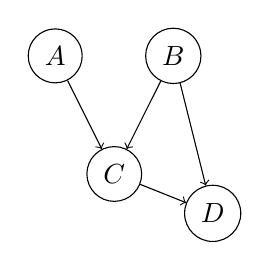
\begin{tikzpicture}
	\draw (0,0) node[shape=circle, draw=black](a){$A$};
	\draw (1.5,0) node[shape=circle, draw=black](b){$B$};
	\draw (0.75,-1.5) node[shape=circle, draw=black](c){$C$};
	\draw (2,-2) node[shape=circle, draw=black](d){$D$};
	
	\draw [->](a) -- (c);
	\draw [->](b) -- (c);
	\draw [->](b) -- (d);
	\draw [->](c) -- (d);
\end{tikzpicture}
\end{minipage}
\begin{minipage}[c]{0.3\textwidth}
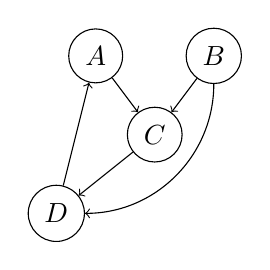
\begin{tikzpicture}

	\draw (0,0) node[shape=circle, draw=black](a){$A$};
	\draw (1.5,0) node[shape=circle, draw=black](b){$B$};
	\draw (0.75,-1.0) node[shape=circle, draw=black](c){$C$};
	\draw (-0.5,-2) node[shape=circle, draw=black](d){$D$};
	
	\draw [->](a) -- (c);
	\draw [->](b) -- (c);
	\draw [->](b.south) to [out=270, in= 0] (d.east);
	\draw [->](c) -- (d);
	\draw [->](d) -- (a);
\end{tikzpicture}
\end{minipage}
\caption{Example of a DAG (left) and a graph with a directed
cycle (right).}
\label{fig:example_DAG}
\end{figure}

Define parents
Define ancestors?

\section{Bayesian networks with DAGs}
What do these DAGs have to do with Bayesian networks? As mentioned
earlier in the context of Bayesian networks they define conditional
independence between variables. Let us first define Bayesian networks:

\begin{defn}[Bayesian networks]

\end{defn}